This section presents a methodology to extract geometric and photometric features of a vehicle's rear side, focusing specifically on the detection of taillights, the localization of the license plate and the localization of the side mirror from image frames. These features serve as critical landmarks for estimating the rear plane and pose of the vehicle in 3D space.

\section{Frames extraction from video}
After filming the nighttime video and calibrating the camera, we moved to extract a set of evenly spaced frames from our video file for further analysis or processing. Specifically, we opened the video, computed the total number of frames, and then selected a fixed number of frames uniformly distributed across the video timeline. We then saved the frames extracted in a folder.

Figure~\ref{fig:frames_sequence} shows four frames extracted from the original video. The symmetric taillights and the license plate are clearly visible across all frames, and serve as key features for 3D localization and orientation estimation.

\begin{figure}[h!]
    \centering
    \begin{subfigure}[b]{0.24\textwidth}
        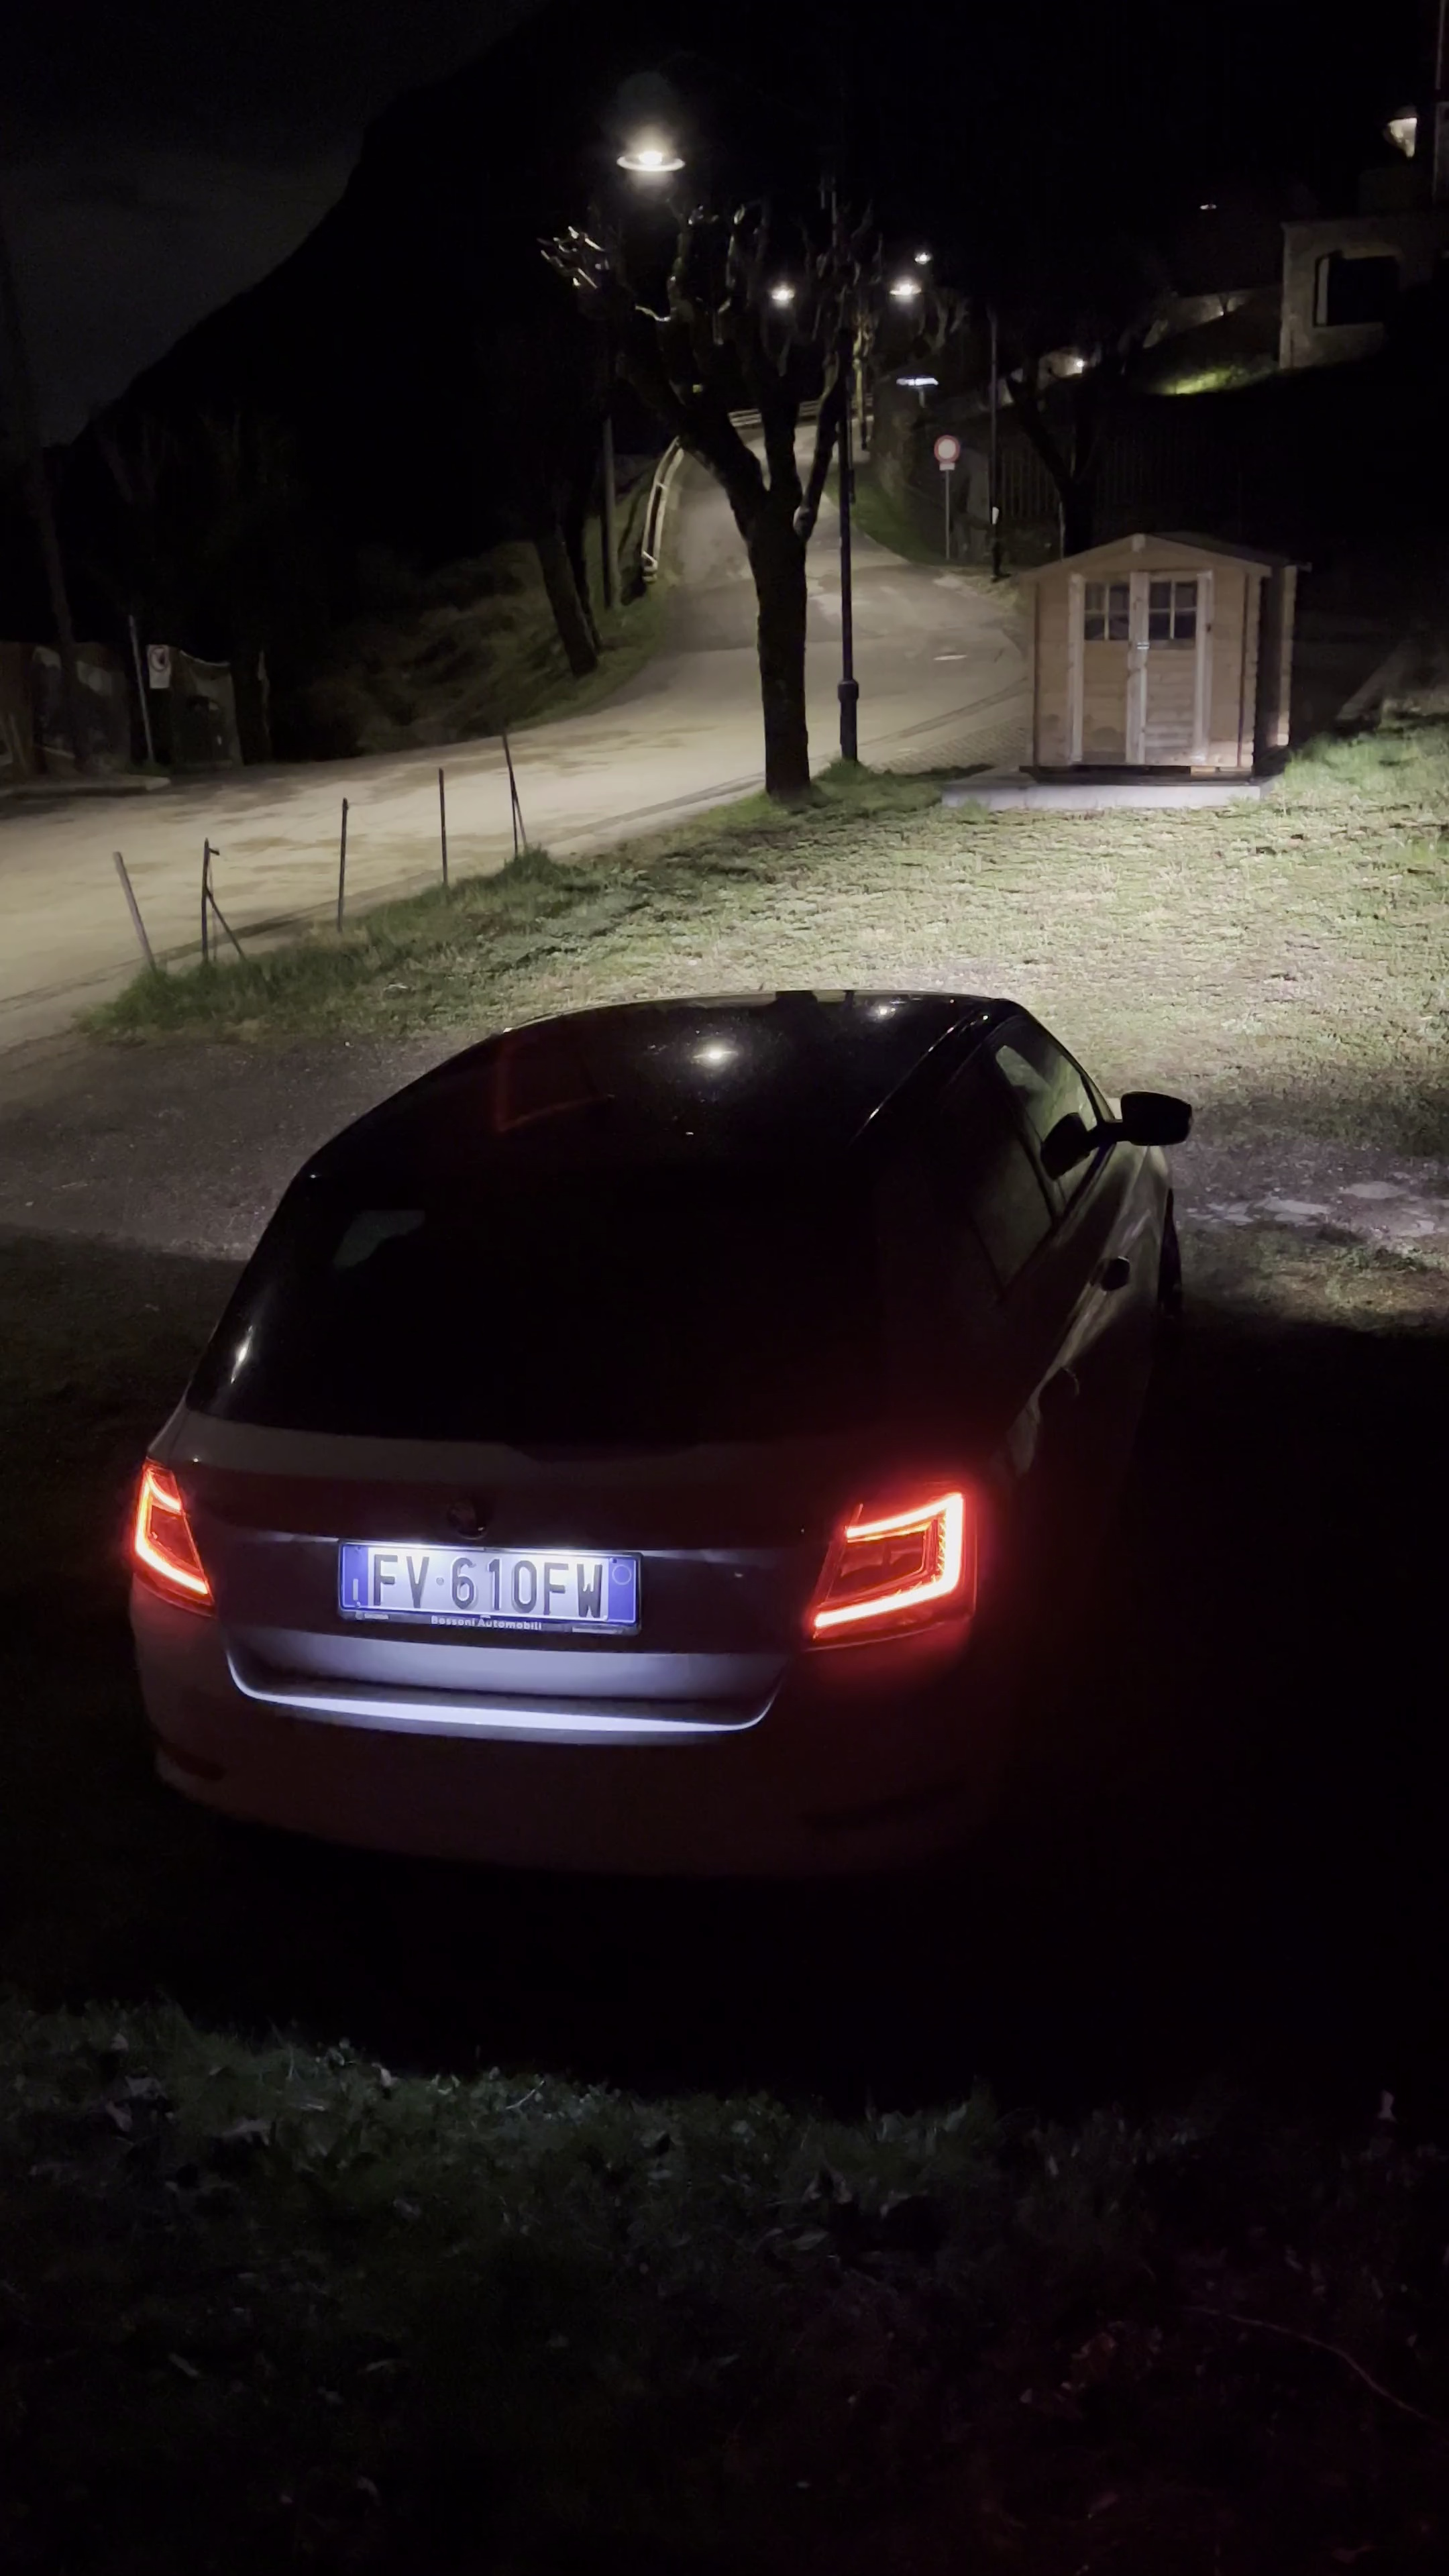
\includegraphics[width=\textwidth]{Images/featureExtractions/frame00.jpg}
        \caption{Frame 0}
    \end{subfigure}
    \begin{subfigure}[b]{0.24\textwidth}
        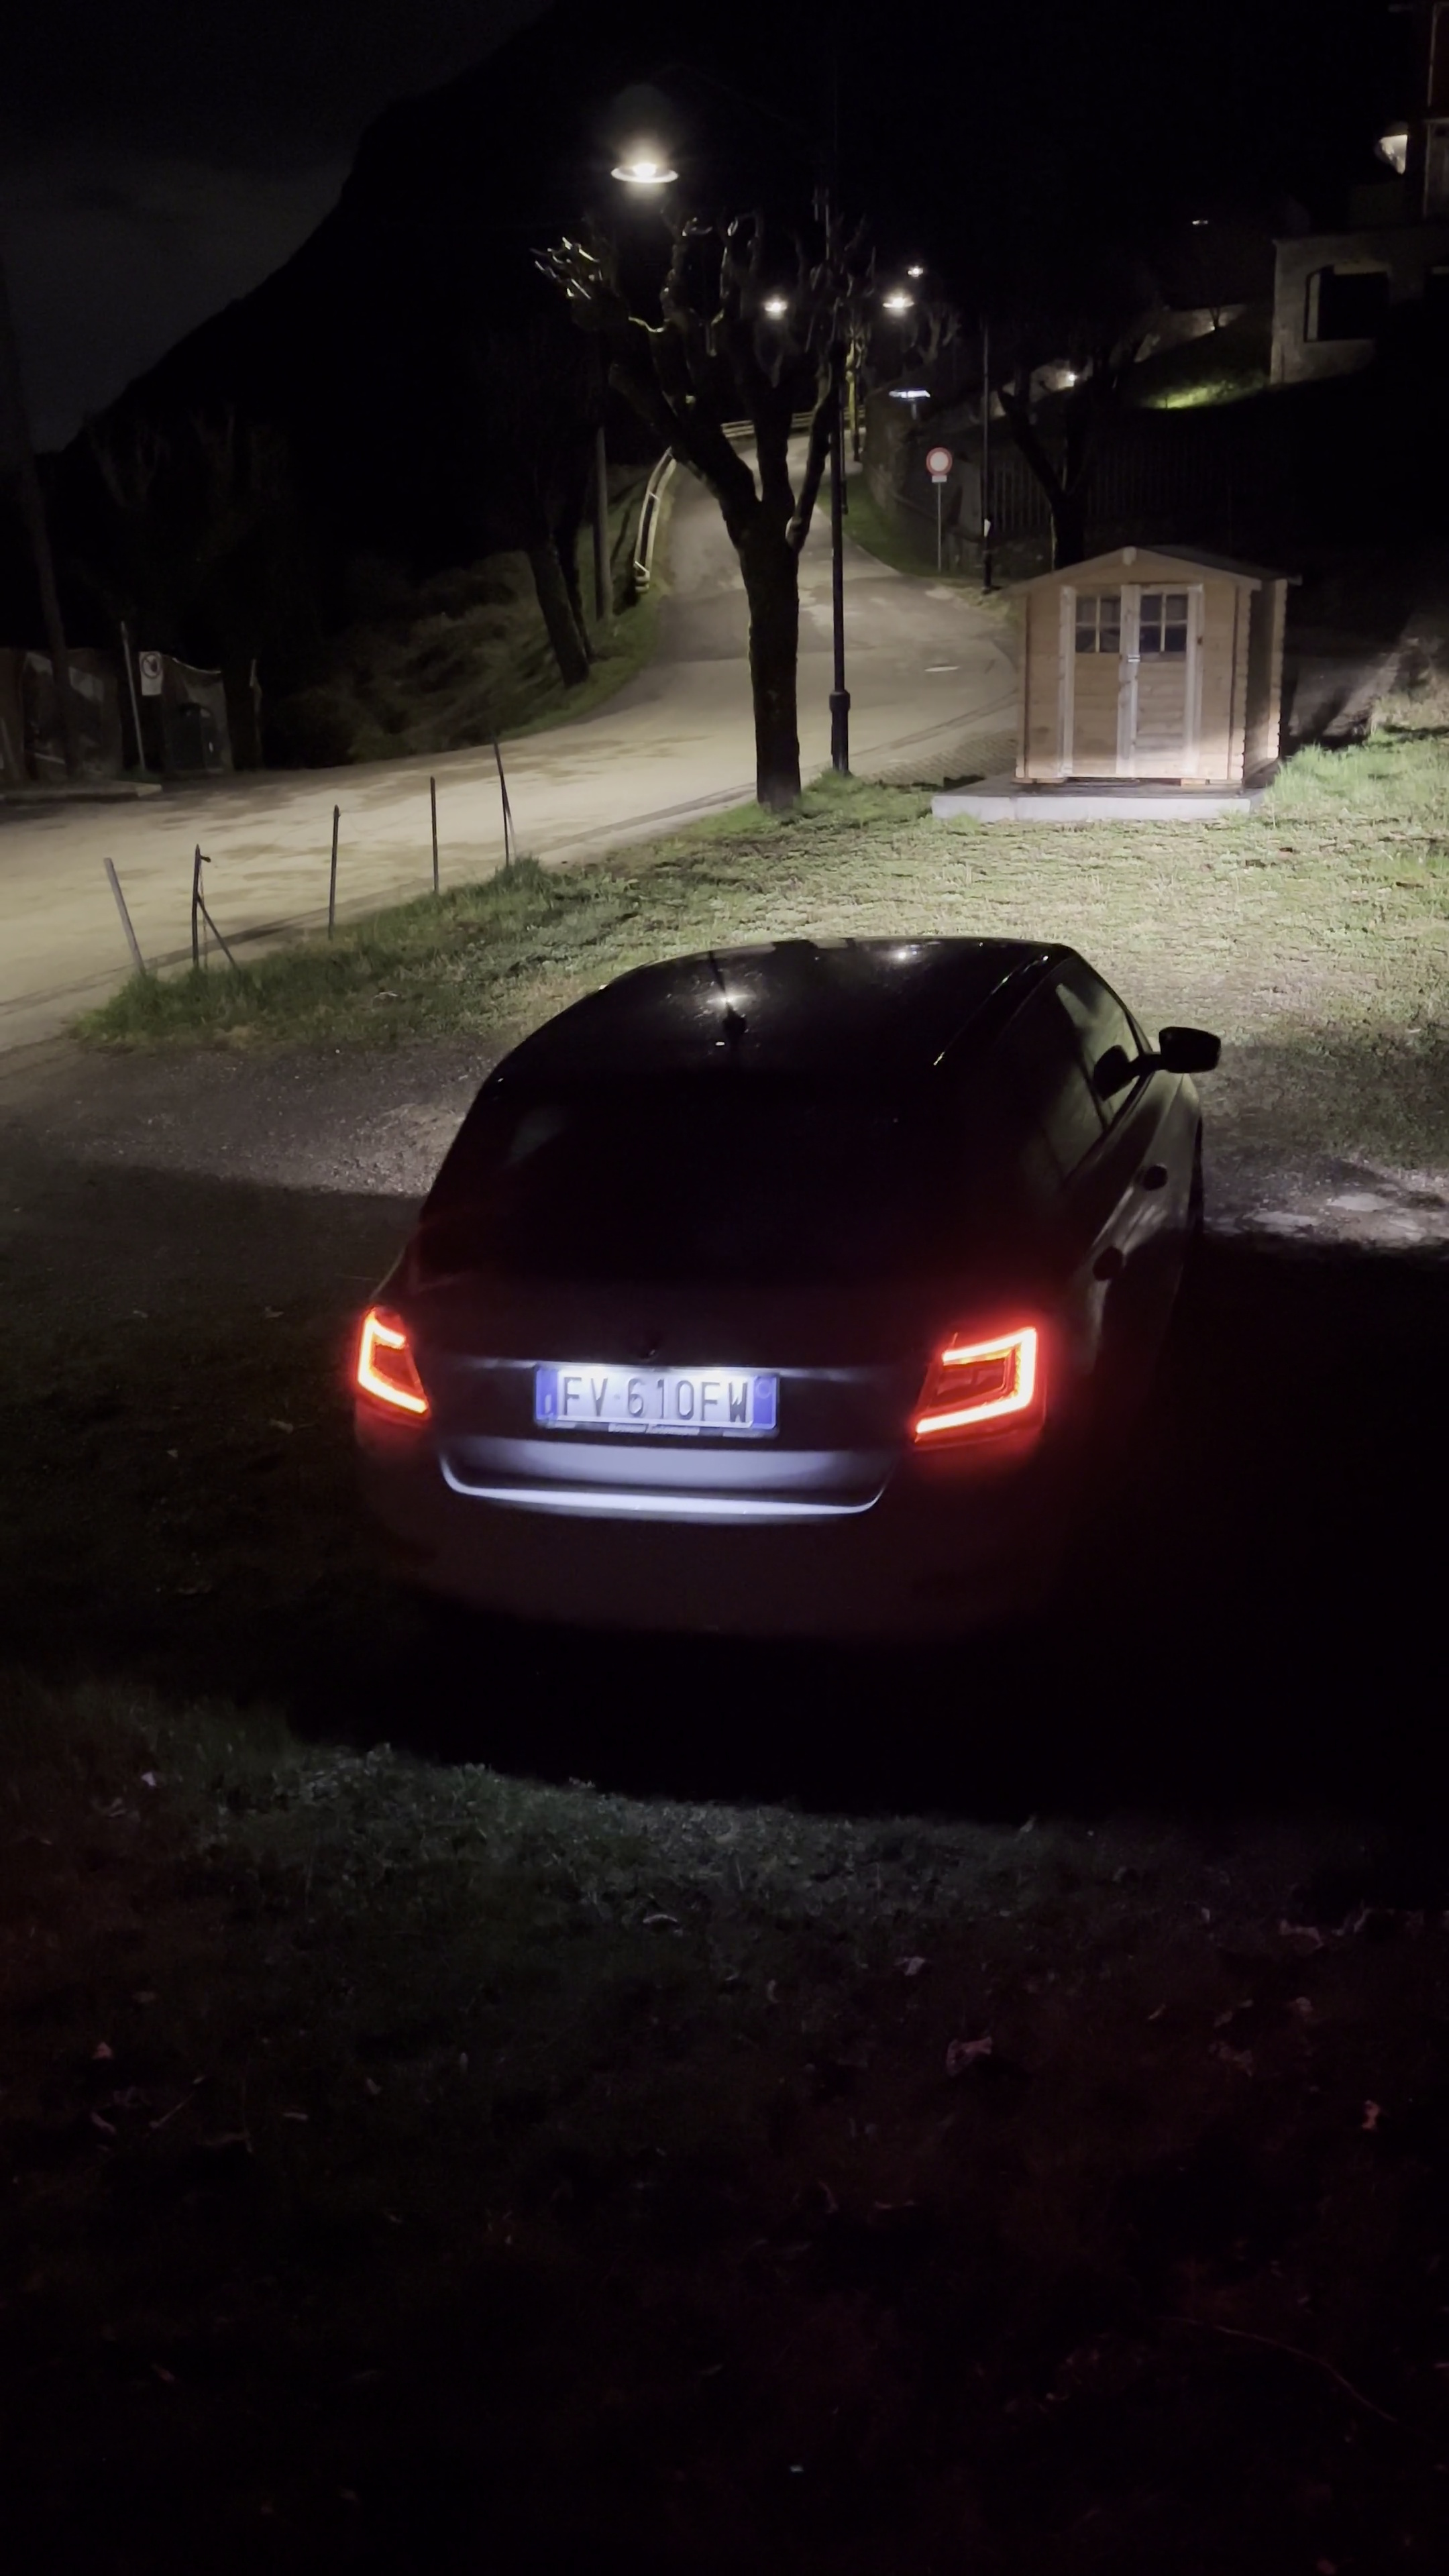
\includegraphics[width=\textwidth]{Images/featureExtractions/frame04.jpg}
        \caption{Frame 4}
    \end{subfigure}
    \begin{subfigure}[b]{0.24\textwidth}
        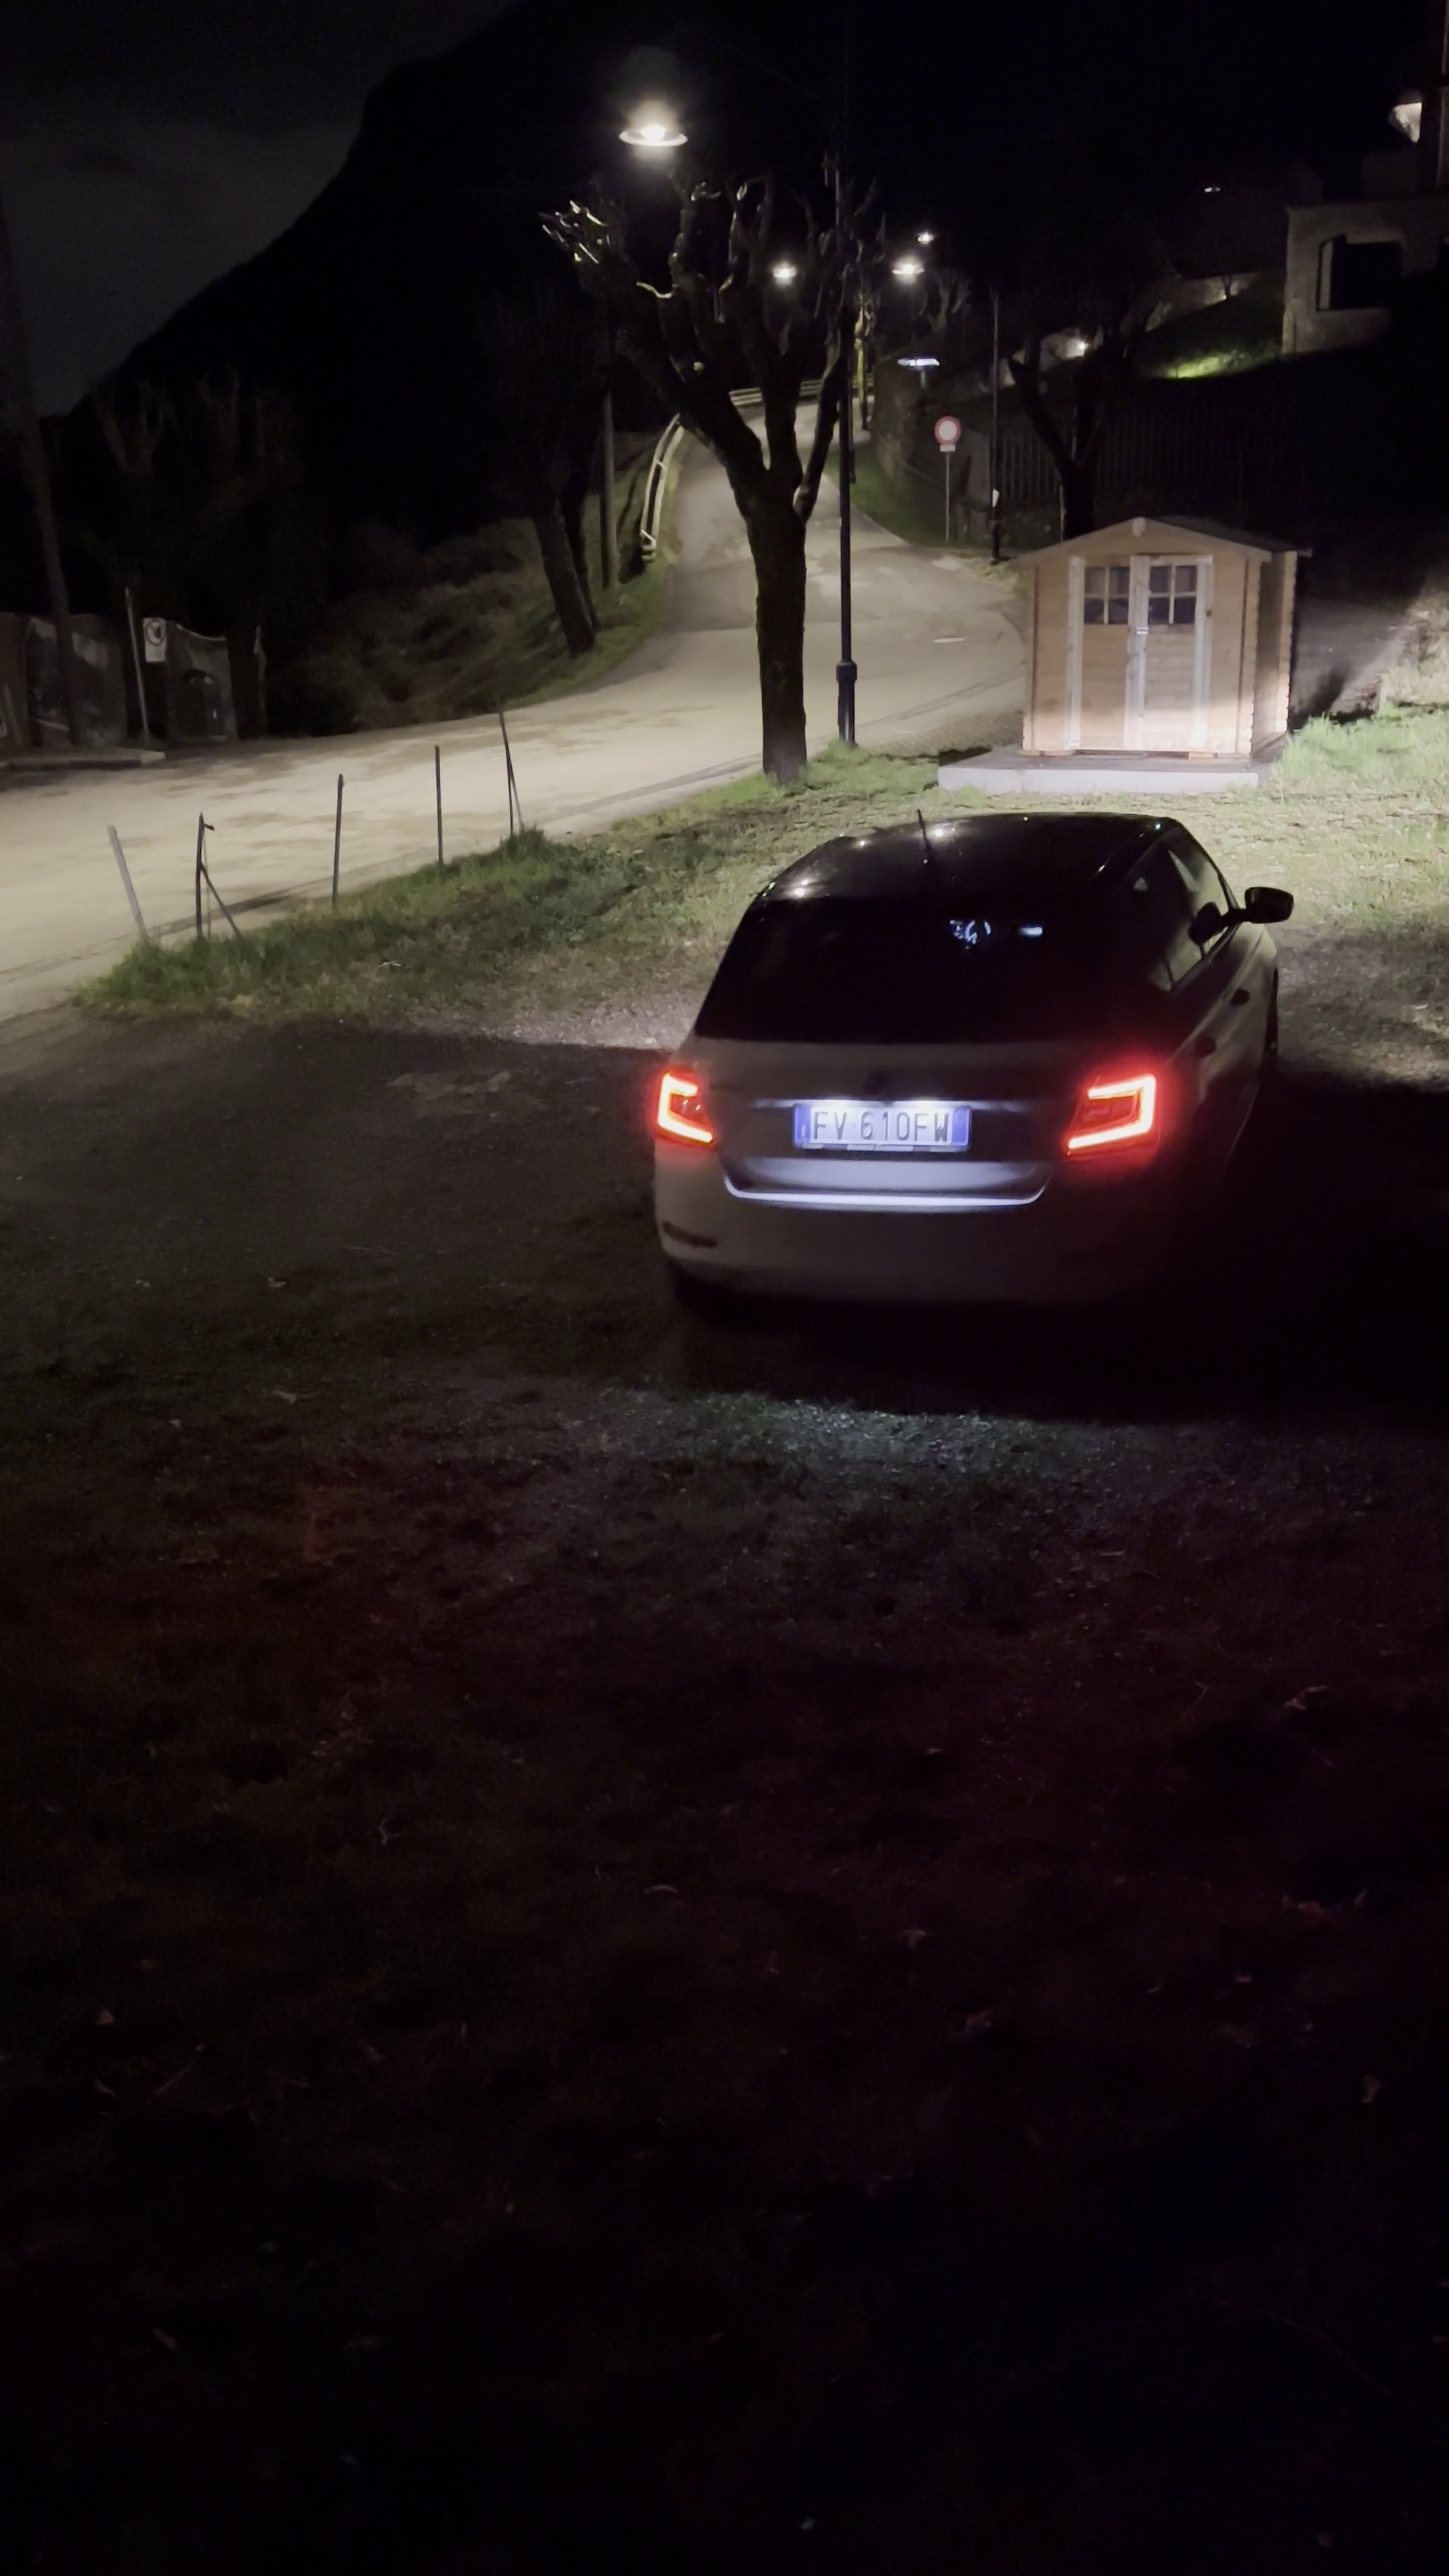
\includegraphics[width=\textwidth]{Images/featureExtractions/frame08.jpg}
        \caption{Frame 8}
    \end{subfigure}
    \begin{subfigure}[b]{0.24\textwidth}
        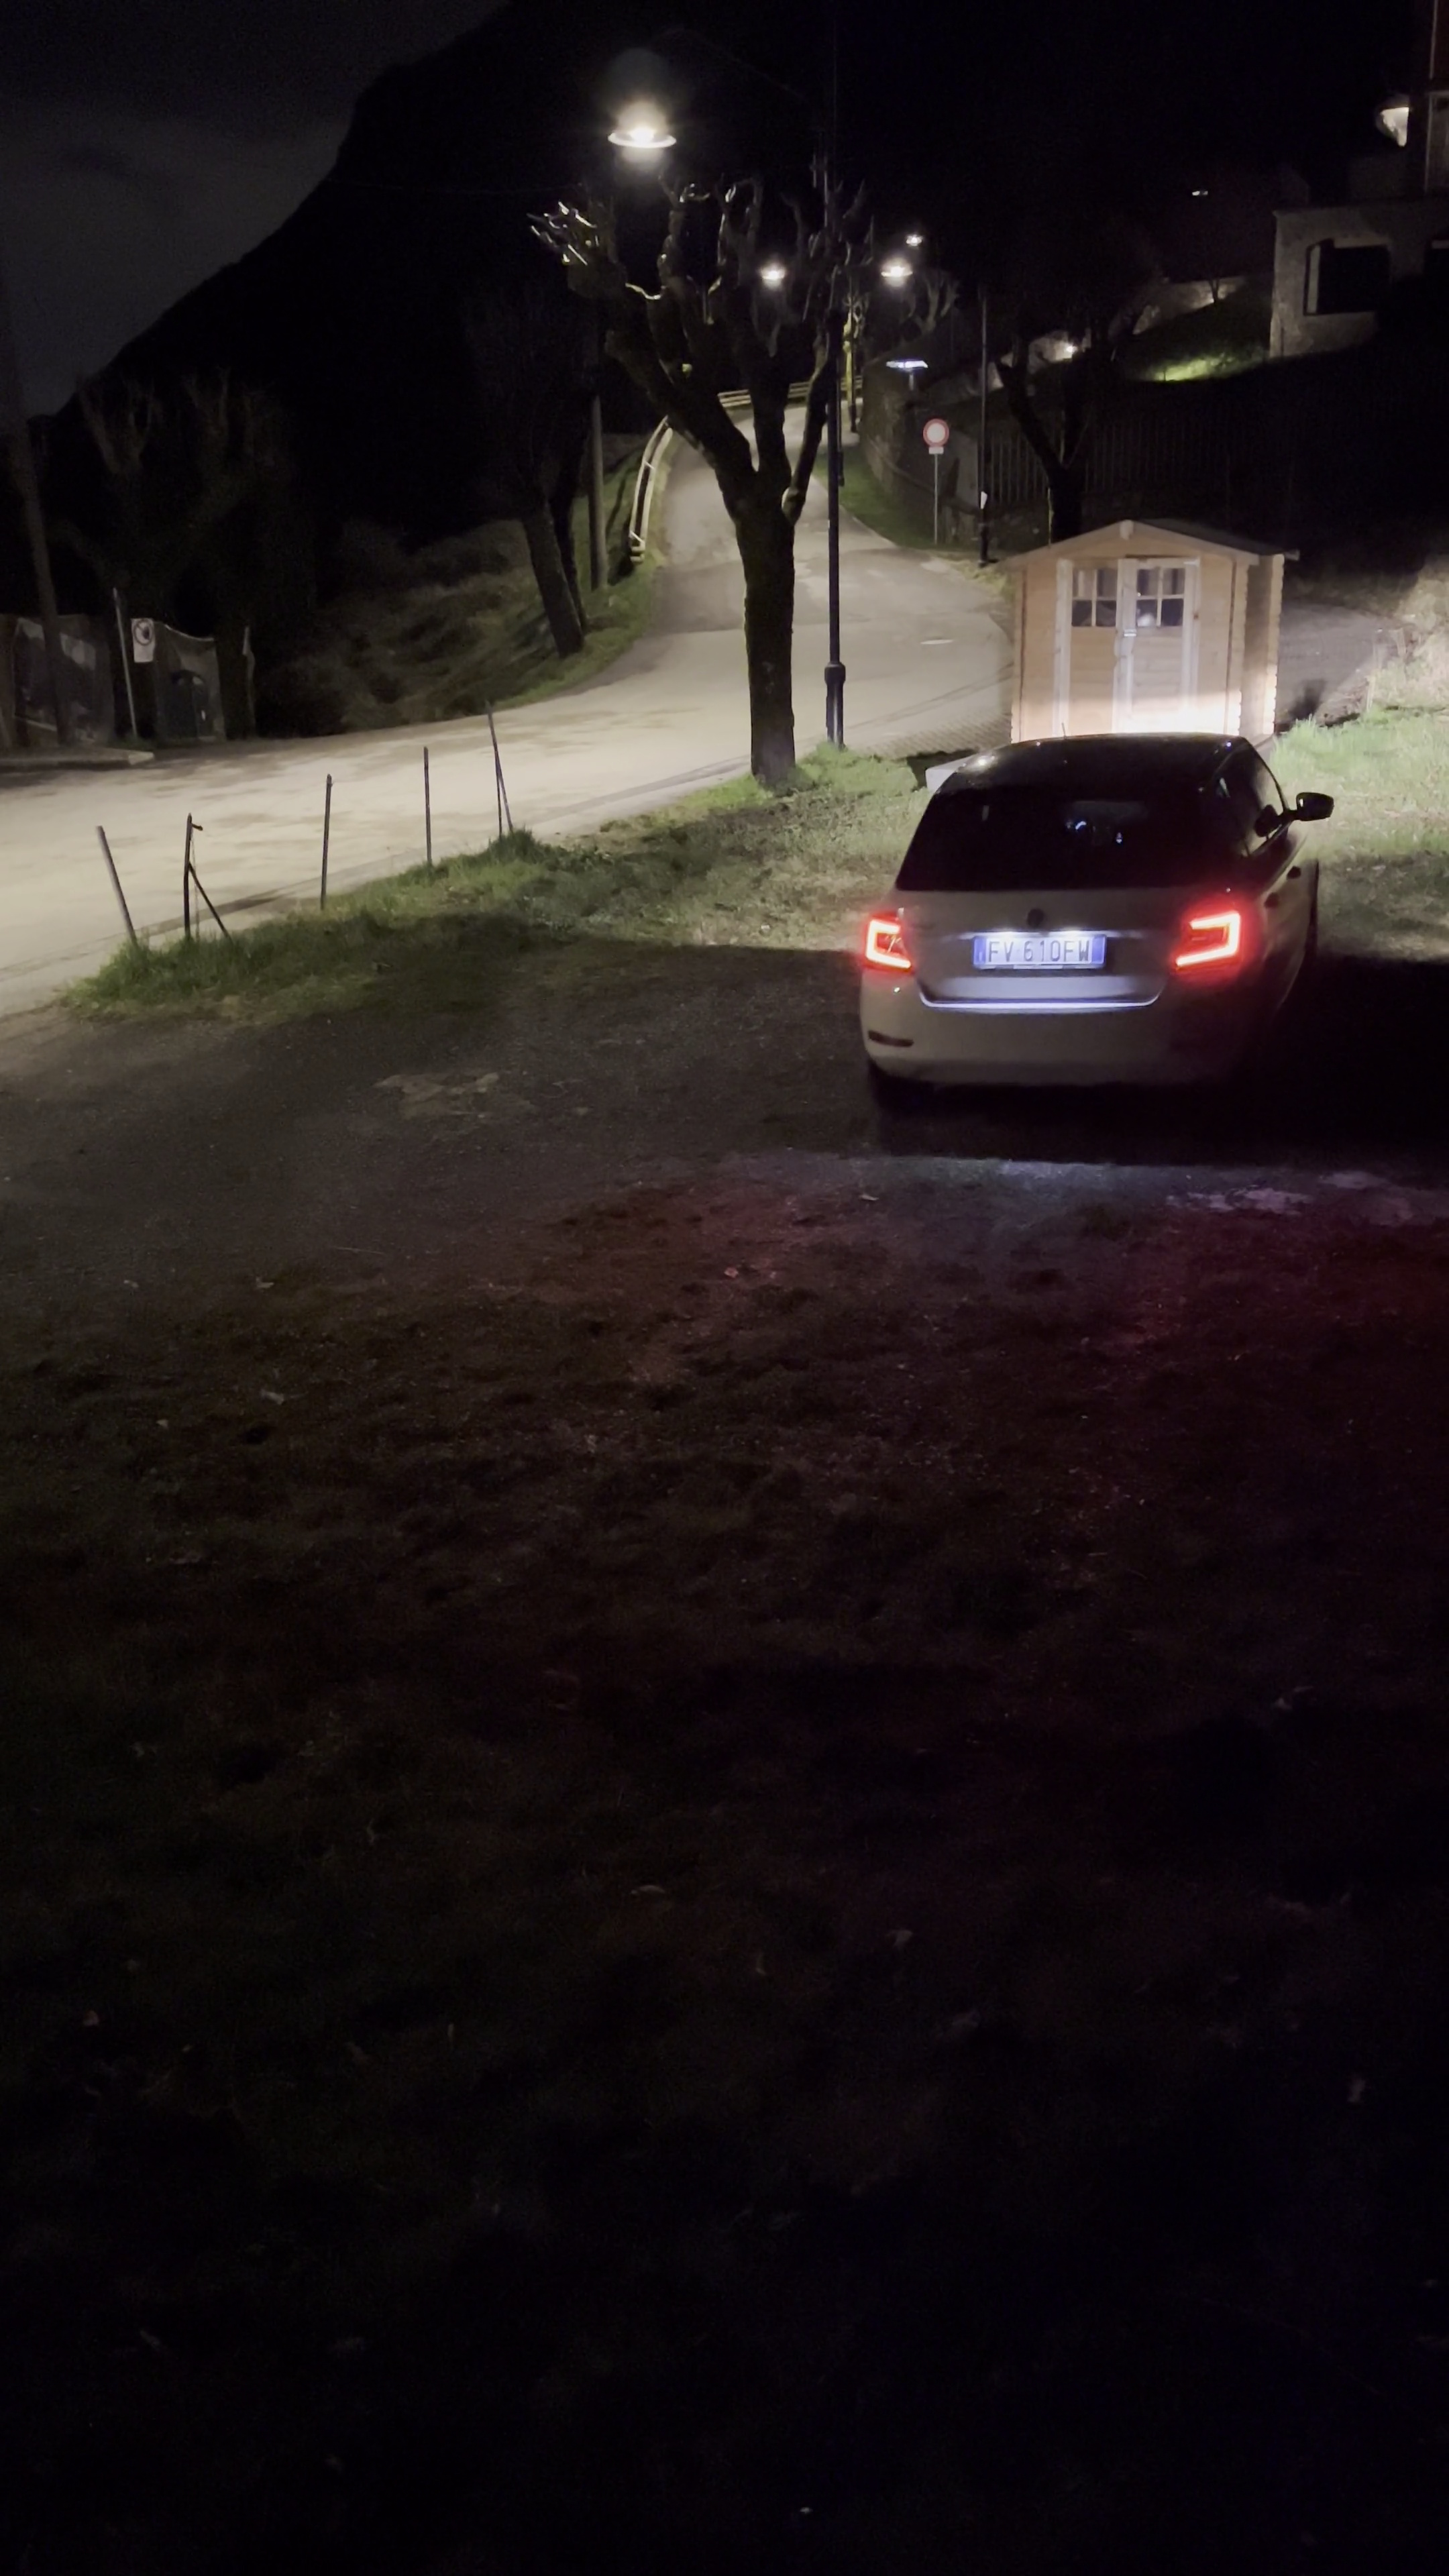
\includegraphics[width=\textwidth]{Images/featureExtractions/frame12.jpg}
        \caption{Frame 12}
    \end{subfigure}

    \caption{Sequence of extracted frames used for symmetric feature tracking}
    \label{fig:frames_sequence}
\end{figure}

\section{Taillights Extraction}
The detection process begins by isolating the vehicle from the background using a convolutional neural network trained on object detection (such as YOLO). This network identifies and localizes the vehicle in each image through a bounding box. The image is then cropped to this bounding box, reducing irrelevant background content and focusing analysis on the vehicle’s rear.

Once the rear of the vehicle has been isolated, we aim at locating the red taillights. Rather than operating in RGB color space, which is sensitive to illumination changes, the image is converted to HSV (Hue, Saturation, Value). This shift is non-trivial: in HSV space, hue represents color in a more stable manner, making red easier to isolate under variable lighting conditions such as shadows, glares, or overexposure.

Two hue ranges are defined—one near 0° and another near 180°—to encompass the dual ends of the red spectrum, since taillights have a stronger red in the heart of lights and a lighter red around them. These ranges are used to create binary masks that isolate red regions. Morphological operations follow, cleaning up the masks by removing small noise and enhancing continuous regions. From here, contours are detected and filtered. The obtained mask looks as follows:

\begin{figure}[htbp]
    \centering
    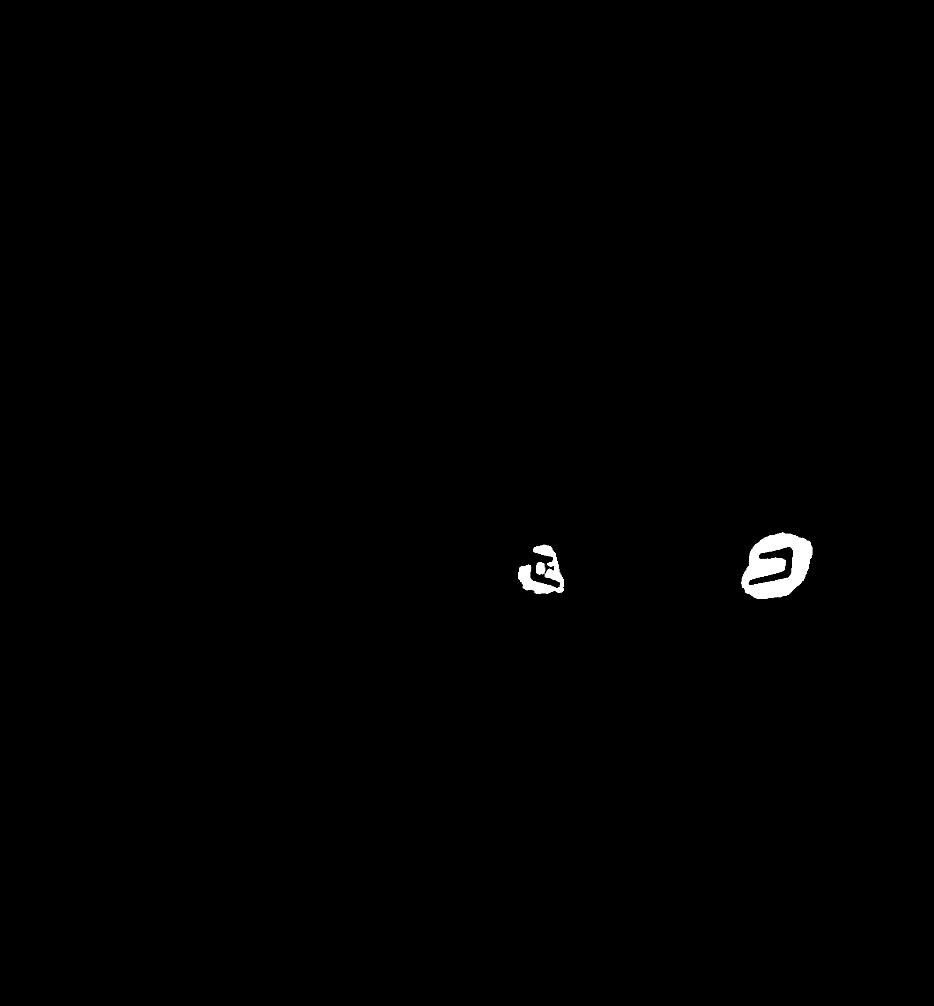
\includegraphics[width=0.5\linewidth]{Images//featureExtractions/redLightsMask.png}
    \caption{Mask found for red taillights}
    \label{fig:redLightsMask}
\end{figure}

The assumption is that the two largest red regions within this refined mask correspond to the taillights. This is a reasonable consideration, especially in urban night driving scenarios where taillights are often the most prominent red features. The methodology then computes two points for each taillight: the center and the bottom outer edge. These points are not are going to serve later as structural anchors for orientation estimation and projection.

\begin{figure}[htbp]
    \centering
    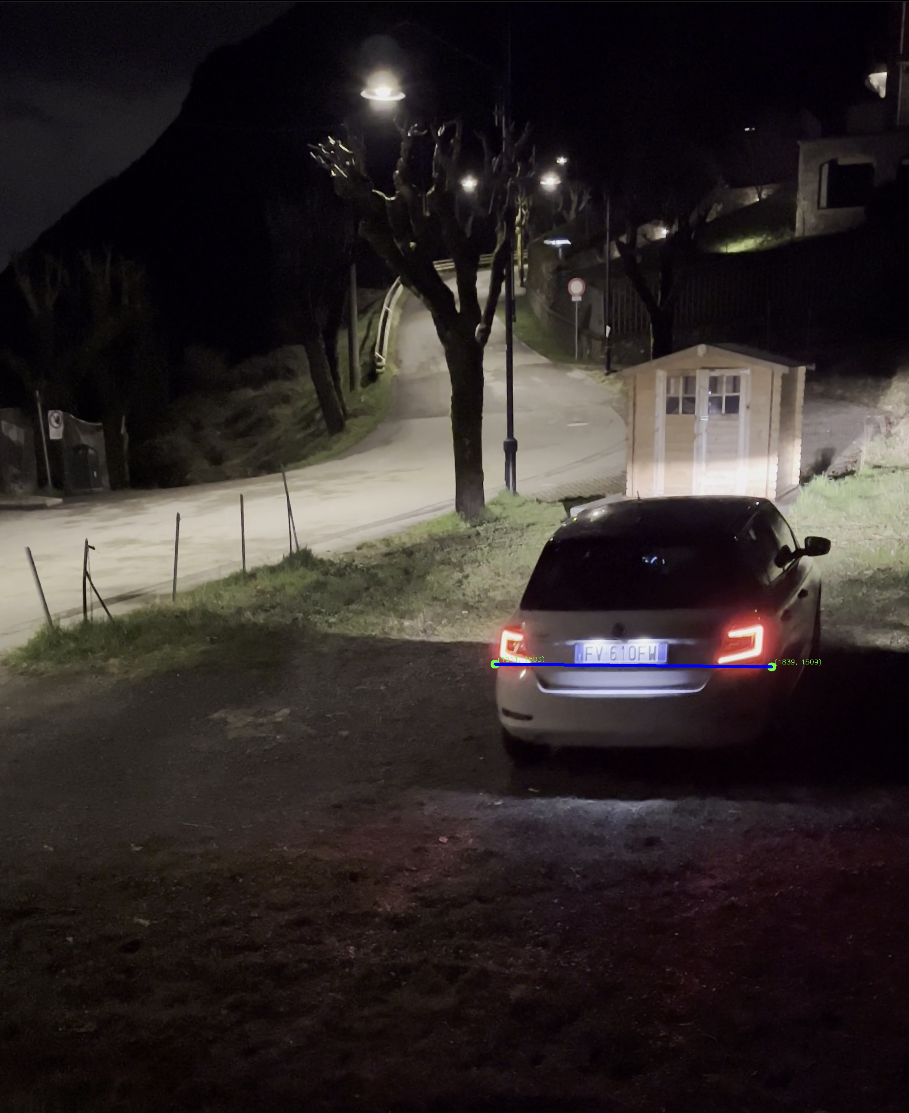
\includegraphics[width=0.4\linewidth]{lightsDetection1.png}
    \caption{Example of taillights detection from a frame}
    \label{fig:lightsDetection}
\end{figure}

Using these taillight detections, the orientation of the rear plane is inferred by calculating the angle of the line joining the taillights. This angle is used to rotate the image such that the taillights lie along a horizontal axis, making subsequent feature extraction more stable and geometrically consistent.

\section{License Plate Extraction}
Following rotation, the license plate is expected to lie directly below the line connecting the taillights. A region of interest (ROI) is defined between and below the taillights to constrain the search space. Within this region, segmentation is performed to isolate the license plate, using its characteristic colour properties—primarily white for the body of the plate and blue for the side strip, as found in many European plates.

\begin{figure}[htbp]
    \centering
    
\includegraphics[width=0.5\linewidth]{Images//featureExtractions/plateMask.png}
    \caption{Mask found for plate}
    \label{fig:plateMask}
\end{figure}

Contours are then extracted and ranked based on geometric properties. Among the candidates, the one with the largest area and an appropriate aspect ratio (typically between 1.5 and 5.5) is selected as the license plate. The bounding box surrounding this contour defines the spatial extent of the plate in the image.

The final output of this process is the localization of the license plate via its bounding box and the precise positions of the taillights. These elements jointly define a consistent geometric configuration on the vehicle’s rear surface and are essential for downstream tasks such as vanishing point estimation, camera resectioning, and 3D back-projection of the rear plane.

\begin{figure}[htbp]
    \centering
    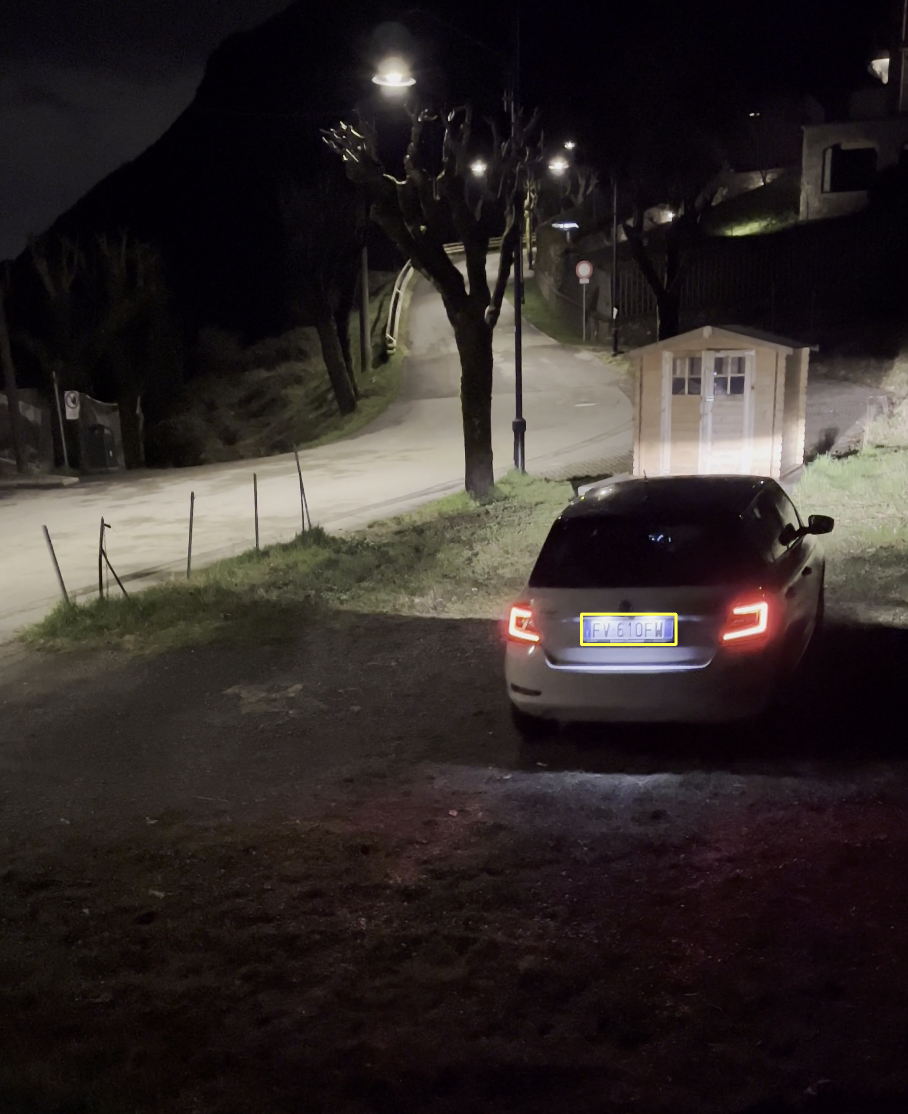
\includegraphics[width=0.4\linewidth]{Images/licenceDetection1.png}
    \caption{Example of licence plate detection from a frame}
    \label{fig:licenceDetection}
\end{figure}

\section{Side Mirror Extraction}
This section outlines a procedure for detecting the side mirror of a vehicle from a single image frame. The mirror serves as a salient lateral landmark that contributes to understanding the vehicle's spatial extent and orientation in 3D space.

The process begins with isolating the vehicle from its surroundings using an object detection model based on the YOLO architecture, as in the previous section. To account for side elements like mirrors that may lie slightly outside the bounding box, the crop is expanded slightly along the horizontal axis.

Once the vehicle region is extracted, the image is preprocessed to highlight structural edges. The cropped frame is first converted to gray-scale, then smoothed using a Gaussian blur to reduce noise. This is followed by Canny edge detection, which enhances high-contrast boundaries and delineates object contours. This step ensures that only well-defined shapes—such as the mirror's outline—are retained for further analysis.

Contours are extracted from the resulting edge map and filtered to retain only those above a certain arc length threshold. This helps eliminate small and irrelevant features while preserving prominent shapes likely to correspond to vehicle components. The filtered contours are then drawn onto a blank canvas for visual inspection and geometric reasoning.

To locate the side mirror, the algorithm searches for the contour point with the most extreme horizontal (x-axis) position. This point is selected based on the assumption that the mirror protrudes outward from the main body of the vehicle and will be positioned near the outermost edge of the cropped frame.

Once identified, the position of the mirror is adjusted to match the coordinates of the original image by reapplying the offset introduced during the initial cropping. This ensures spatial consistency with other detected features.

The output is a single point representing the mirror's location in the global image frame. This point can be integrated with other detected features—such as taillights or license plates—to improve vehicle orientation estimation, determine lateral spread.

\begin{figure}[htbhp]
    \centering
    \begin{subfigure}[b]{0.32\textwidth}
        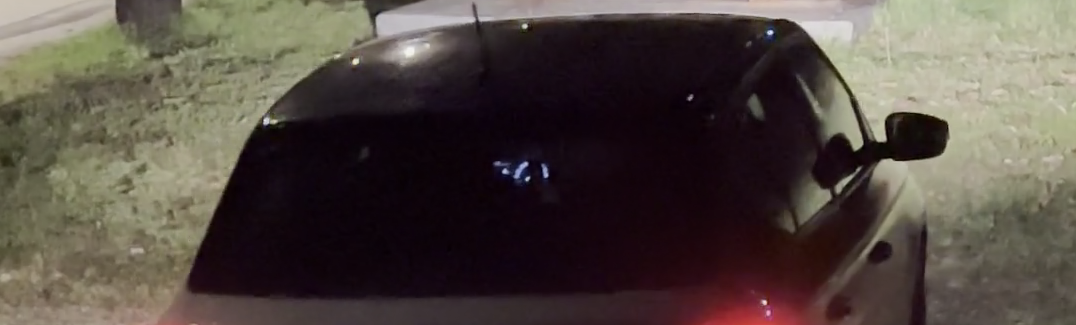
\includegraphics[width=\textwidth]{Images/featureExtractions/MirrorDetection/yolo_frame1.png}
        \caption{Cropped part}
    \end{subfigure}
    \begin{subfigure}[b]{0.32\textwidth}
        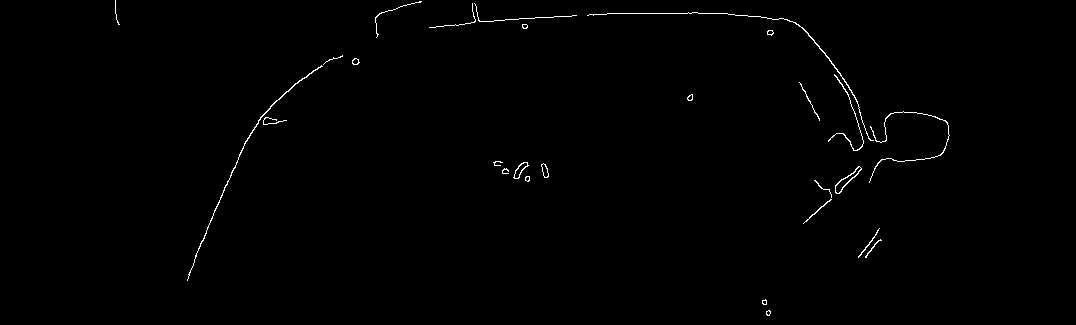
\includegraphics[width=\textwidth]{Images/featureExtractions/MirrorDetection/edges.png}
        \caption{Edges Detected}
    \end{subfigure}
    \begin{subfigure}[b]{0.32\textwidth}
        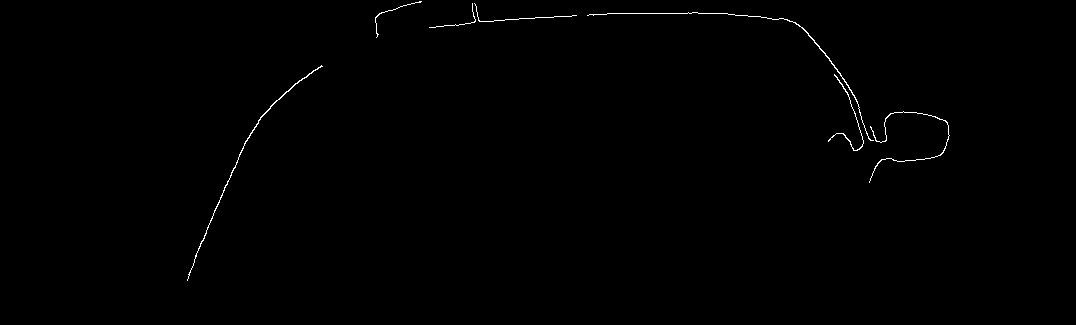
\includegraphics[width=\textwidth]{Images/featureExtractions/MirrorDetection/long_contours.png}
        \caption{Filtered Edges}
    \end{subfigure}

    \caption{Intermediate steps of side mirror detection}
    \label{fig:side-mirror-steps}
\end{figure}

\begin{figure}[htbhp]
    \centering
    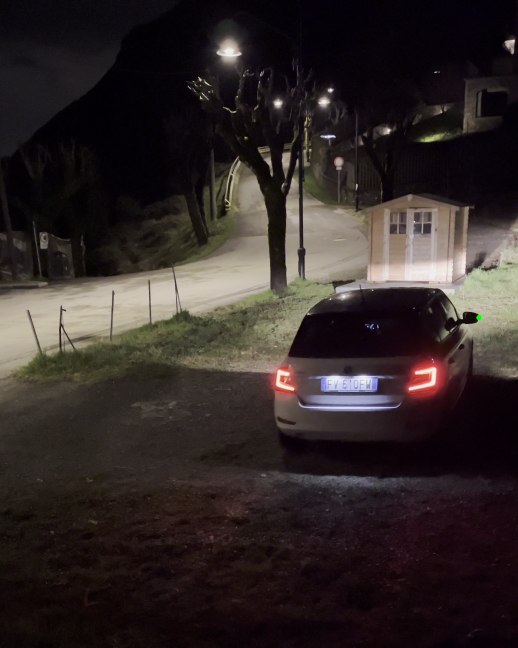
\includegraphics[width=0.4\linewidth]{Images/featureExtractions/MirrorDetection/mirror_detected.png}
    \caption{Example of side mirror detection from a frame}
    \label{fig:mirrorDetection}
\end{figure}
